\begin{figure}[htb]
    \centering
    \subfloat[quality]{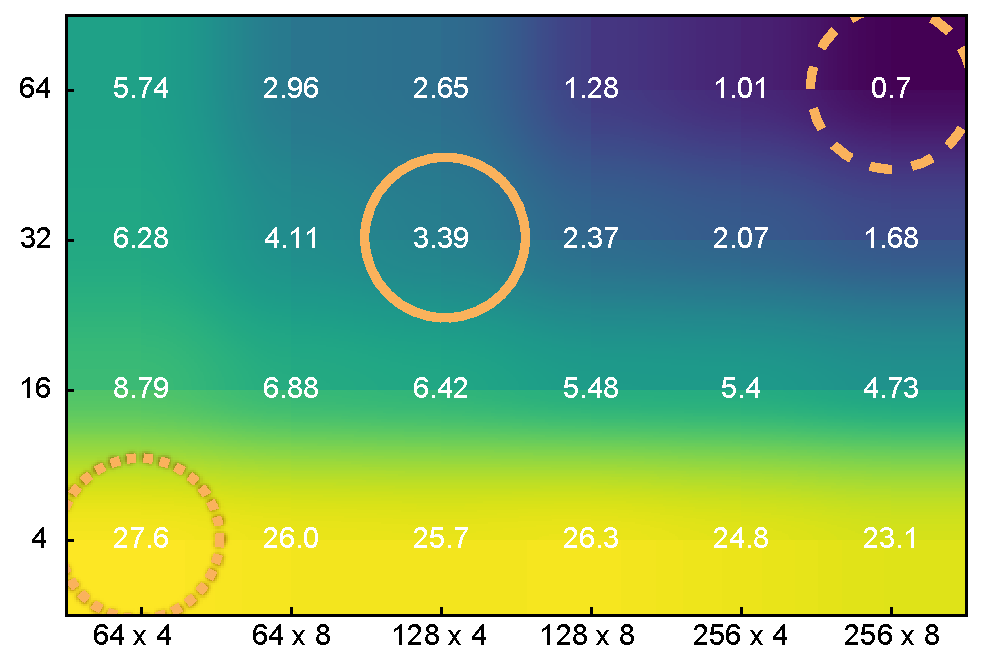
\includegraphics[width=0.48\linewidth]{TOG/figs/latency_vs_quality/heat_quality2.pdf}\label{fig:optimization:heat:quality}}
    \subfloat[latency]{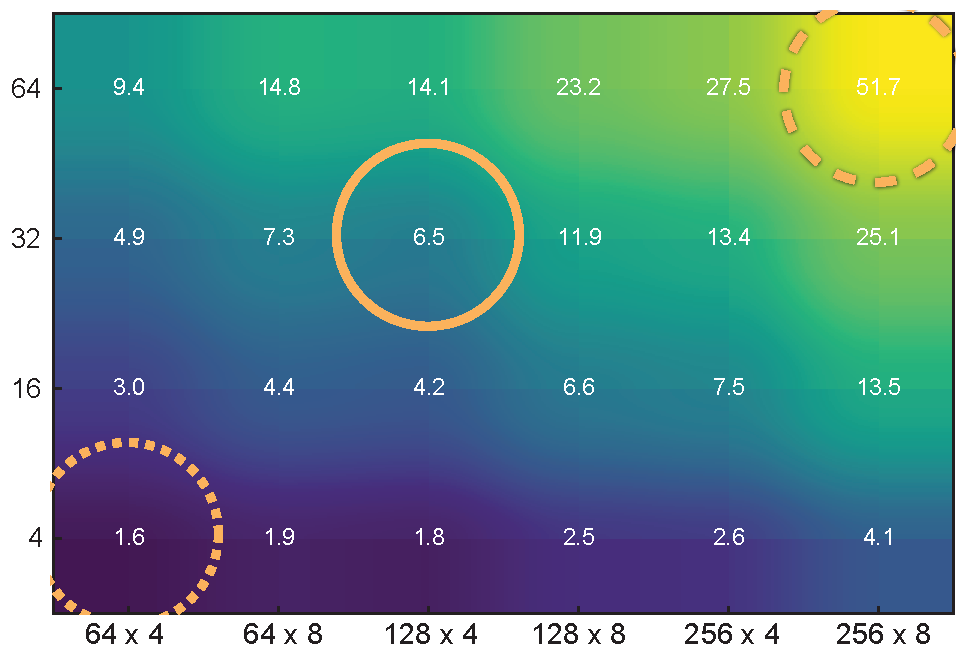
\includegraphics[width=0.48\linewidth]{TOG/figs/latency_vs_quality/heat_time2.pdf}\label{fig:optimization:heat:time}}
    
    \subfloat[quality-only]{
\includegraphics[width=0.3\linewidth]{TOG/figs/latency_vs_quality/quality_only.pdf}\label{fig:optimization:quality}}\hspace{0.5em}
    \subfloat[latency-only]{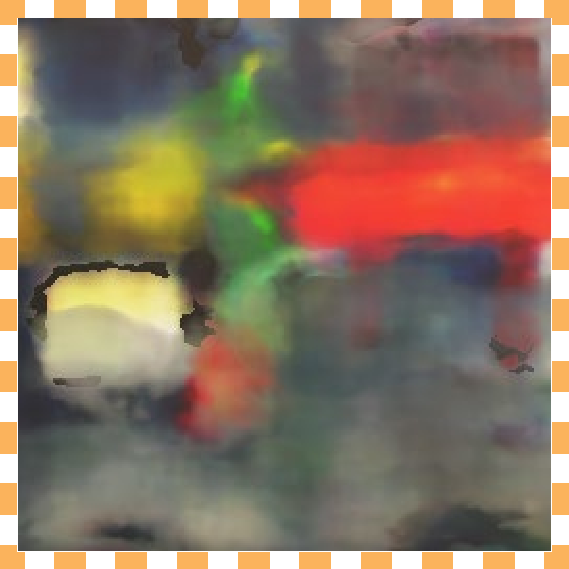
\includegraphics[width=0.3\linewidth]{TOG/figs/latency_vs_quality/latency_only.pdf}\label{fig:optimization:time}}\hspace{0.5em}
    \subfloat[ours]{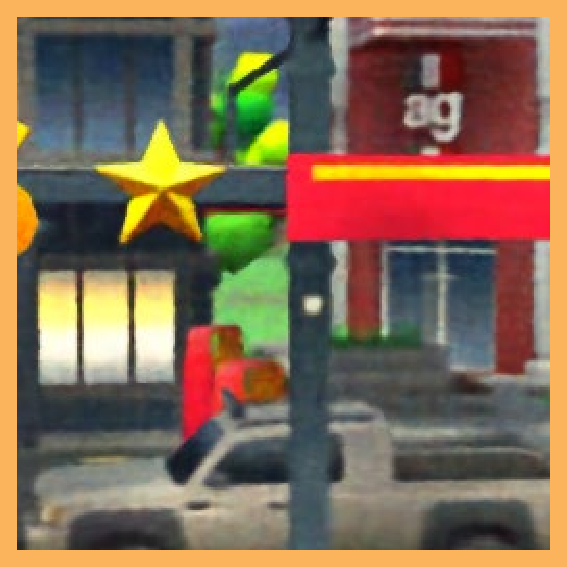
\includegraphics[width=0.3\linewidth]{TOG/figs/latency_vs_quality/our.pdf}\label{fig:optimization:our}}
    \Caption{Latency-quality joint-optimization.}
    {%
    \protect\subref{fig:optimization:heat:quality}/\protect\subref{fig:optimization:heat:time} shows \protect\Cref{eq:imageError}/latency(in millisecond under pytorch implementation) of an example foveal network.
    The values are computed with various settings of $\mlpLayerNum\times\mlpChannelNum$ (x-axis) and $\sphereNum$ (y-axis). The second row indicates a corresponding foveal image under different settings. Our method balances both perceptual quality and latency.\nothing{\qisun{(Jan 24) What is the unit of \subref{fig:optimization:heat:time}? It shouldn't be second, right?}\dnc{It's millisecond.}}%nothing
    }
    \label{fig:optimization}
\end{figure}